\documentclass{article}

\usepackage{polski}
\usepackage[utf8]{inputenc}
\usepackage{graphicx}
\usepackage{url}


\title{Praca inżynierska}
\date{2017-10-01}
\author{Jędrzej Kozal, Karol Szpila}

\begin{document}

\begin{titlepage}
	\centering
	
\includegraphics[width=0.25\textwidth]{logo_pol_wroclaw.png}\par\vspace{1cm}
	{\scshape\LARGE Politechnika Wrocławska \par}
	\vspace{1cm}
	{\scshape\Large E-media\par}
	\vspace{1.5cm}
	{\huge\bfseries Sprawozdanie z projektu \par}
	\vspace{2cm}
	{\Large\itshape Karol Szpila, Jędrzej Kozal\par}
	\vfill
	prowadzący\par
	Dr hab.~Wojciech \textsc{Bożejko}, prof. nadzw. PWr

	\vfill

% Bottom of the page
	{\large 2017-10-01\par}
\end{titlepage}

	
\section{Wstęp}
Celem pierwszej części projektu jest wczytanie nagłówka wybranego pliku dźwiękowego i graficznego oraz wykonanie transformaty Fouriera wczytanego pliku. W omawianym projekcie zrealizowano odczyt nagłówków plików z rozszerzeniem wav oraz bmp.

\subsection{Wykorzystane narzędzia}
Zadanie projektowe zrealizowano w języku Python w wersji 2.7. Decyzja ta były podyktowana głównie szybkością tworzenia kodu, oraz prostotą tego języka. Do realizacji graficznego interfejsu użytkownika wykorzystano framework kivy. Do wyświetlania wyniku transformaty Fouriera wykorzystano bibliotekę matplotlib.

\section{Omówienie struktury i zawartości nagłówków}

\subsection{Strukutra nagłówka plików .wav}

Nagłówek pliku wav jest podzielony na trzy części (ang. chunks): "RIFF", "fmt" oraz "data". Każda część zaczyna się od czteroznakowego kontrolnego tagu (ChunkID). Zgodnie z formatem RIFF każda część musi zawierać tag kontrolny, oraz rozmiar (ilość bajtów) części. Dodatkowo wszystkie tagi są zakodowane w big endian, wszystkie pozostałe dane są zakodowane w little endian. Pierwsza część zawiera długość całego pliku oraz jego format. Druga część zawiera wszystkie parametry opisujące plik. Trzecia część zawiera dane - zbiór sampli.


\begin{figure} 
\centering
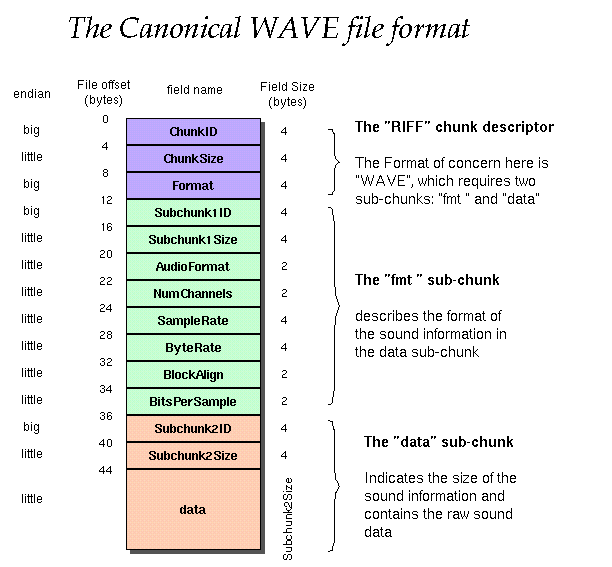
\includegraphics[width=15cm]{wav-sound-format.png}
\caption{Schemat nagłówka pliku wav. Źródło: http://soundfile.sapp.org/doc/WaveFormat/}
\end{figure}

\subsubsection{Omówienie poszczególnych parametrów}

\subparagraph{AudioFormat}
Dla LPCM (Linear Pulse-Code Modulation) parameter ten przyjmuje wartość 1. Inna wartość oznacza inną formę kodowania sampli.

\subparagraph{NumChannels}
Ilość kanałów. Dla mono przyjmuje wartość 1, dla stereo przyjmuje wartość 2. Parametr może przyjmować dowolną wartość do 65535. Niektóre programy wykorzystują ten fakt do przechowywania różnych sygnałów nie będących dźwiękiem (np. LTspice przechowuje kształty różnych sygnałów).

\subparagraph{SampleRate}
Ilość próbek na sekundę - częstotliwość próbkowania.

\subparagraph{ByteRate}
Ilość bajtów na sekundę. Wartość można wyrazić wzorem:
\begin{equation}
ByteRate = SampleRate * NumChannels * BitsPerSample/8
\end{equation}

\subparagraph{BlockAlign}
Parametr przyjmuje następujące wartości: 1 - 8 bit mono, 2 - 8 bit stereo/16 bit mono, 4 - 16 bit stereo.
\begin{equation}
BlockAlign = NumChannels * BitsPerSample/8
\end{equation}

\subparagraph{BitsPerSample}
Ilość bitów przypadających na jedną próbkę.


\subsection{Strukutra nagłówka plików .bmp}

Pliku bmp jest podzielony na następujące części: nagłówek pliku, nagłówek DIB, tablica kolorów, tablica pikseli, profil kolorów ICC. W ramach zadania projektowego przeczytano i zweryfikowano poprawność pierwsze 54 bajty, co odpowiada następującym własnościom:

\subparagraph{FileSize}
Rozmiar całego pliku.

\subparagraph{Offset}
Wartość offsetu dla której rozpoczyna się tablica pikseli w pliku.

\subparagraph{SizeOfBitmapHeader}
Rozmiar nagłówka pliku, musi przyjmnować wartości większe bądź równe 40.

\subparagraph{BitmapWidth}
Szerokość bitmapy w pikselach.

\subparagraph{BitmapHeight}
Wysokość bitmapy w pikselach.

\subparagraph{NumberOfColorPlains}
Ilość płaszczyzn przechowywanych w pliku. Parametr ten musi być równy 1.

\subparagraph{BitCount}
Ilość bitów na piksel. Dopuszczalne wartości: 1, 4, 8, 16, 24, lub 32. W zależności od tego parametru sposób przechowywania kolorów jest inny: dla 8 lub mniej wartości wszystkich kolorów są przechowywane w tablicy kolorów, dla więcej niż 8 jasność dla każdego kanału RGB jest przechowywana dla każdego piksela osobno (tablica kolorów nie istnieje), dla wartości 16 lub 32 wartości kolorów są przechowywane w polach bitowych, każdy kolor posiada swoje bity, wartość koloru dla poszczególnych kanałów jest obliczana na podstawie zbioru trzech masek bitowych.

\subparagraph{Compression}
Rodzaj kompresji. Przyjmowane wartości 0 - brak kompresji, 1 - RLE-8, 2 - RLE-4 (Run-Length Encoding - metoda kompresji bezstratnej, polegająca na zastąpieniu ciągu znaków ilością ich powtórzeń) lub 3 - pola bitowe

\subparagraph{SizeImage}
Rozmiar w bajtach przechowywanych pikseli. Przyjmuje wartość zero dla obrazu bez kompresji.

\subparagraph{XPelsPerMeter}
Pionowa rozdzielczość pliku. Wartość w pikselach na metr.

\subparagraph{YPelsPerMeter}
Pozioma rozdzielczość pliku. Wartość w pikselach na metr.

\subparagraph{ClrUsed}
Ilość kolorów, które faktycznie zostały użyte lub zero. Wykorzystanie tego parametru pozwala na skrócenie wielkości tablicy kolorów, co wpływa na wielkość całego pliku (zwłaszcza dla plików o większym BitCount.

\subparagraph{ClrImportant}
Liczba istotnych kolorów, które mogą zostać użyte lub zero. Jeśli obraz jest wyświetlany na gorszej jakości ekranie, pozwala to określić jakie kolory powinny zostać wykorzystane. W tym celu w tablicy kolorów najbardziej istotne kolory powinny być przechowywane jako pierwsze.



\subsection{Sposób realizacji zadania, szczegóły implementacyjne}
W projekcie wszczególniono klasy, odpowiadające za poszczególne aspekty projektu. Przy projektowaniu struktury klas w projekcie kierowano się prostotą oraz łatwą rozszerzalnością. Projekt nie został zrealizowany w metodyce clean code, ponieważ wymagałoby to większego nakładu na refaktoryzację istniejących rozwiązań. Dodatkowo w stworzonym kodzie można się doszukać niezgodności z dobrymi praktykami programowania obiektowego takimi jak SOLID. Przykładem może być zasada pojedyńczej odpowiedzialności, która nie jest przestrzegana w projekcie w celu zachowania prostoty kodu. Ponadto warto nadmienić że inżynieria oprogramowania nie jest głównym aspektem tego projektu.
Do przechowywania zawartości nagłówka pliku została stworzona klasa Header. Klasa ta przechowuje słownik, zawierający nazwy poszczególnych pól z nagłówka oraz wczytane wartości. Zdecydowano na ten sposób przechowywania informacji ze względu na łatwą rozszerzalność projektu - nagłówki różnych plików mogą być reprezentowane przez tą samą klasę.

Do operacji odczytu nagłówka pliku wykorzystano wzorzec budowniczy. W założeniu wzorzec ten ma formalizować proces tworzenia skomplikowanych obiektów. Podobną odpowiedzialność posiada wzorzec projektowy fabryka abstrakcyjna. Odpowiada on za tworzenie skomplikowanego obiektu z odpowiedniej "rodziny". 

Biorąc pod uwagę podstawione zadanie wykorzystanie tego wzorca wydaje się być właściwym wyborem, jednakże konstrukcja klasy Header umożliwiła na zastosowanie innego rozwiązania. Zaimplementowano klasę HeaderBuilder będącą klasą bazową dla klas odpowiedzialnych za czytanie konkretnego  nagłówka. Klasa ta posiada metodę $read\_header()$, która przyjmuje nazwę pliku jako parametr, następnie otwiera go, wywołuje metodę $build()$, następnie zamyka plik. Metoda $build()$ jest implementowana w klasach pochodnych, przyjmuje jako parametr otwarty plik, następnie czyta z niego nagłówek i resztę pliku, oraz zwraca wczytany nagłówek oraz dane stanowiące resztę pliku.

W trakcie odczytu pliku w GUI na podstawie rozszerzenia wybranego pliku zostaje podjęta decyzja jaka klasa powinna zostać wykorzystana.

\begin{figure} 
\centering
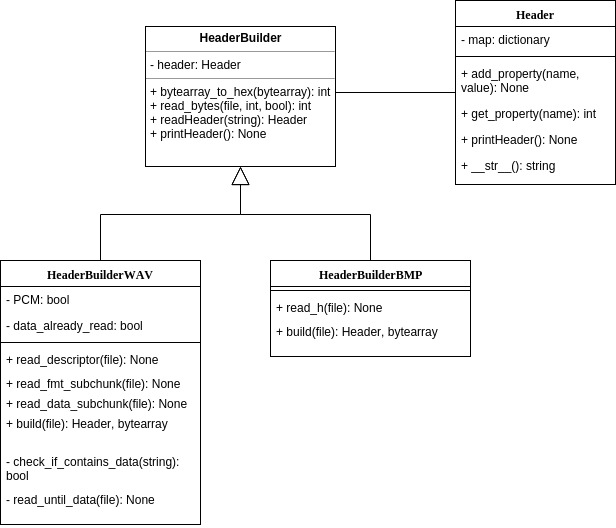
\includegraphics[width=10cm]{Untitled_Diagram.jpg}
\caption{Diagram wykorzystanych klas}
\end{figure}


\newpage
\begin{thebibliography}{9}

\bibitem{wav} 
Specyfikacja nagłówka pliku wav,
\\\texttt{http://soundfile.sapp.org/doc/WaveFormat}

\bibitem{bmpB} 
Zawartość nagłówka pliku bmp,
\\\texttt{http://fastgraph.com/help/bmp\_header\_format.html}

\bibitem{bmp} 
Opis parametrów nagłówka pliku bmp,
\\\texttt{http://www.dragonwins.com/domains/getteched/bmp/bmpfileformat.htm}

\bibitem{kivy}
Dokumentacja biblioteki kivy,
\\\texttt{https://kivy.org/docs/guide/basic.html}

\end{thebibliography}


\end{document}